\documentclass[conference]{IEEEtran}

\usepackage{amsmath,amssymb}
\usepackage{graphicx}
\usepackage{booktabs}
\usepackage{multirow}
\usepackage{hyperref}
\usepackage[utf8]{inputenc}

\graphicspath{{figures/}}

\begin{document}

\title{Predictive KV Cache Amortization for Edge Language Model Inference on Mobile Devices}

\author{
\begin{tabular}[t]{c@{\hspace{4em}}c}
\begin{tabular}[t]{c}
\textbf{Arjit Tripathi}\\
\textit{\small arjit.tripathi2023@vitstudent.ac.in}
\end{tabular} &
\begin{tabular}[t]{c}
\textbf{Heer Shah}\\
\textit{\small shah.heer2023@vitstudent.ac.in}
\end{tabular} \\[1.5em]
\begin{tabular}[t]{c}
\textbf{Medha Sriram}\\
\textit{\small medha.sriram2023@vitstudent.ac.in}
\end{tabular} &
\begin{tabular}[t]{c}
\textbf{Dr.~Shalini~L}\\
\textit{\small l.shalini@vit.ac.in}
\end{tabular}
\end{tabular}
}

\maketitle

% ===========================================================================
% ABSTRACT
% ===========================================================================
\begin{abstract}
On-device language models prepend environmental context prompts before generating responses, but this prefill phase scales as $O(N)$ with prompt length and dominates latency on mobile hardware. We present Context-Aware Predictive KV-Cache Priming (CAP-KVC), which uses environmental sensor signals---GPS, BLE proximity, and time of day---to predict the needed context and pre-compute key-value cache tensors during idle periods. At inference time, the cached state is restored in 2.74~ms, bypassing the context prefill entirely. On a OnePlus~11R with Qwen2.5-0.5B-Instruct (Q4\_K\_M), native-side \texttt{std::chrono} instrumentation confirms a \textbf{40.78$\times$ prefill-specific speedup} (343~ms vs.\ 14001~ms at $N \approx 500$ tokens) and a 4.24$\times$ end-to-end reduction (4574~ms vs.\ 19408~ms). The system is implemented as an Android application with a C++/JNI inference backend based on \texttt{llama.cpp}, a bounded LRU cache manager supporting three simultaneous KV states within 118.7~MB native heap, and sensor-driven context routing with hysteresis-gated drift detection. A proof-of-concept multimodal intent layer (sEMG + gaze, late fusion) is evaluated on synthetic data and does not constitute clinical validation.
\end{abstract}

\begin{IEEEkeywords}
Key-value cache, edge inference, predictive caching, large language model, mobile systems, Android.
\end{IEEEkeywords}

% ===========================================================================
% I. INTRODUCTION
% ===========================================================================
\section{Introduction}
\label{sec:introduction}

Quantized sub-billion-parameter language models now run on mobile SoCs~\cite{dettmers2022,frantar2022,llamacpp}, but context-aware inference---where an environmental system prompt is prepended to the user's input---introduces an $O(N)$ prefill cost that can dominate latency for prompts of several hundred tokens~\cite{vaswani2017}. Applications requiring low-latency contextual responses, such as augmentative communication (AAC) devices~\cite{beukelman2020}, cannot tolerate this overhead.

Server-side KV cache reuse techniques---prefix sharing~\cite{sglang}, paged attention~\cite{vllm}, prompt caching~\cite{cachegen}---exploit multi-tenant request streams unavailable on single-user edge devices, where each request typically reprocesses the full context.

We present \textbf{Context-Aware Predictive KV-Cache Priming (CAP-KVC)}, which decouples the prefill from the inference path on mobile hardware. CAP-KVC uses GPS, BLE proximity, and time-of-day signals to predict the needed semantic context, executes the prefill during idle periods, serializes the resulting KV cache to persistent storage, and restores it in under 3~ms at inference time. The system is implemented as a complete Android application with a C++/JNI backend based on \texttt{llama.cpp}~\cite{llamacpp}, Kotlin orchestration for cache residency and sensor routing, and a proof-of-concept multimodal intent layer. The contributions are:

\begin{enumerate}
    \item A predictive KV cache architecture achieving a 40.78$\times$ prefill-specific speedup and 4.24$\times$ end-to-end speedup on a OnePlus~11R (Qwen2.5-0.5B-Instruct Q4\_K\_M, 343~ms vs.\ 14001~ms prefill, 4574~ms vs.\ 19408~ms end-to-end), with 2.74~ms cache restoration.

    \item An edge-native Android implementation with a scalar-only JNI boundary (9 native functions), reentrant-lock concurrency, and an LRU cache manager bounded to 3 KV states within 118.7~MB native heap.

    \item A deterministic sensor-driven context routing engine with reliability-adaptive weighting and hysteresis-gated drift detection.
\end{enumerate}

% ===========================================================================
% II. RELATED WORK
% ===========================================================================
\section{Related Work}
\label{sec:related}

\textbf{KV cache optimization.}
Token-level compression methods---Scissorhands~\cite{scissorhands}, H$_2$O~\cite{h2o}, SnapKV~\cite{snapkv}, StreamingLLM~\cite{streamingllm}, KVQuant~\cite{kvquant}---reduce within-sequence memory but operate within a single sequence. Server-side prefix reuse systems (SGLang RadixAttention~\cite{sglang}, PagedAttention~\cite{vllm}, Prompt Cache~\cite{promptcache}, CacheBlend~\cite{cacheblend}) and cross-session streaming (CacheGen~\cite{cachegen}, InfiniGen~\cite{infinigen}) target cloud serving with shared request streams. CAP-KVC differs by using environmental sensor signals for cache state selection on a single edge device, where no shared request stream is available.

\textbf{Edge LLM deployment.}
Post-training quantization~\cite{dettmers2022,frantar2022}, architecture-aware design~\cite{mobilellm}, and inference frameworks~\cite{llamacpp,mlcllm} enable on-device execution. PowerInfer-2~\cite{powerinfer2} extends to 47B parameters via heterogeneous NPU/CPU scheduling. Alizadeh et~al.~\cite{llminaflash} use flash memory for models exceeding DRAM capacity. Despite these runtime improvements, the $O(N)$ prefill remains a latency bottleneck when contextual prompts span hundreds of tokens.

% ===========================================================================
% III. SYSTEM DESIGN
% ===========================================================================
\section{System Design}
\label{sec:methodology}

CAP-KVC amortizes contextual prompt ingestion by executing it as a background process prior to user interaction. Fig.~\ref{fig:architecture} presents the system architecture.

\begin{figure*}[t]
\centering
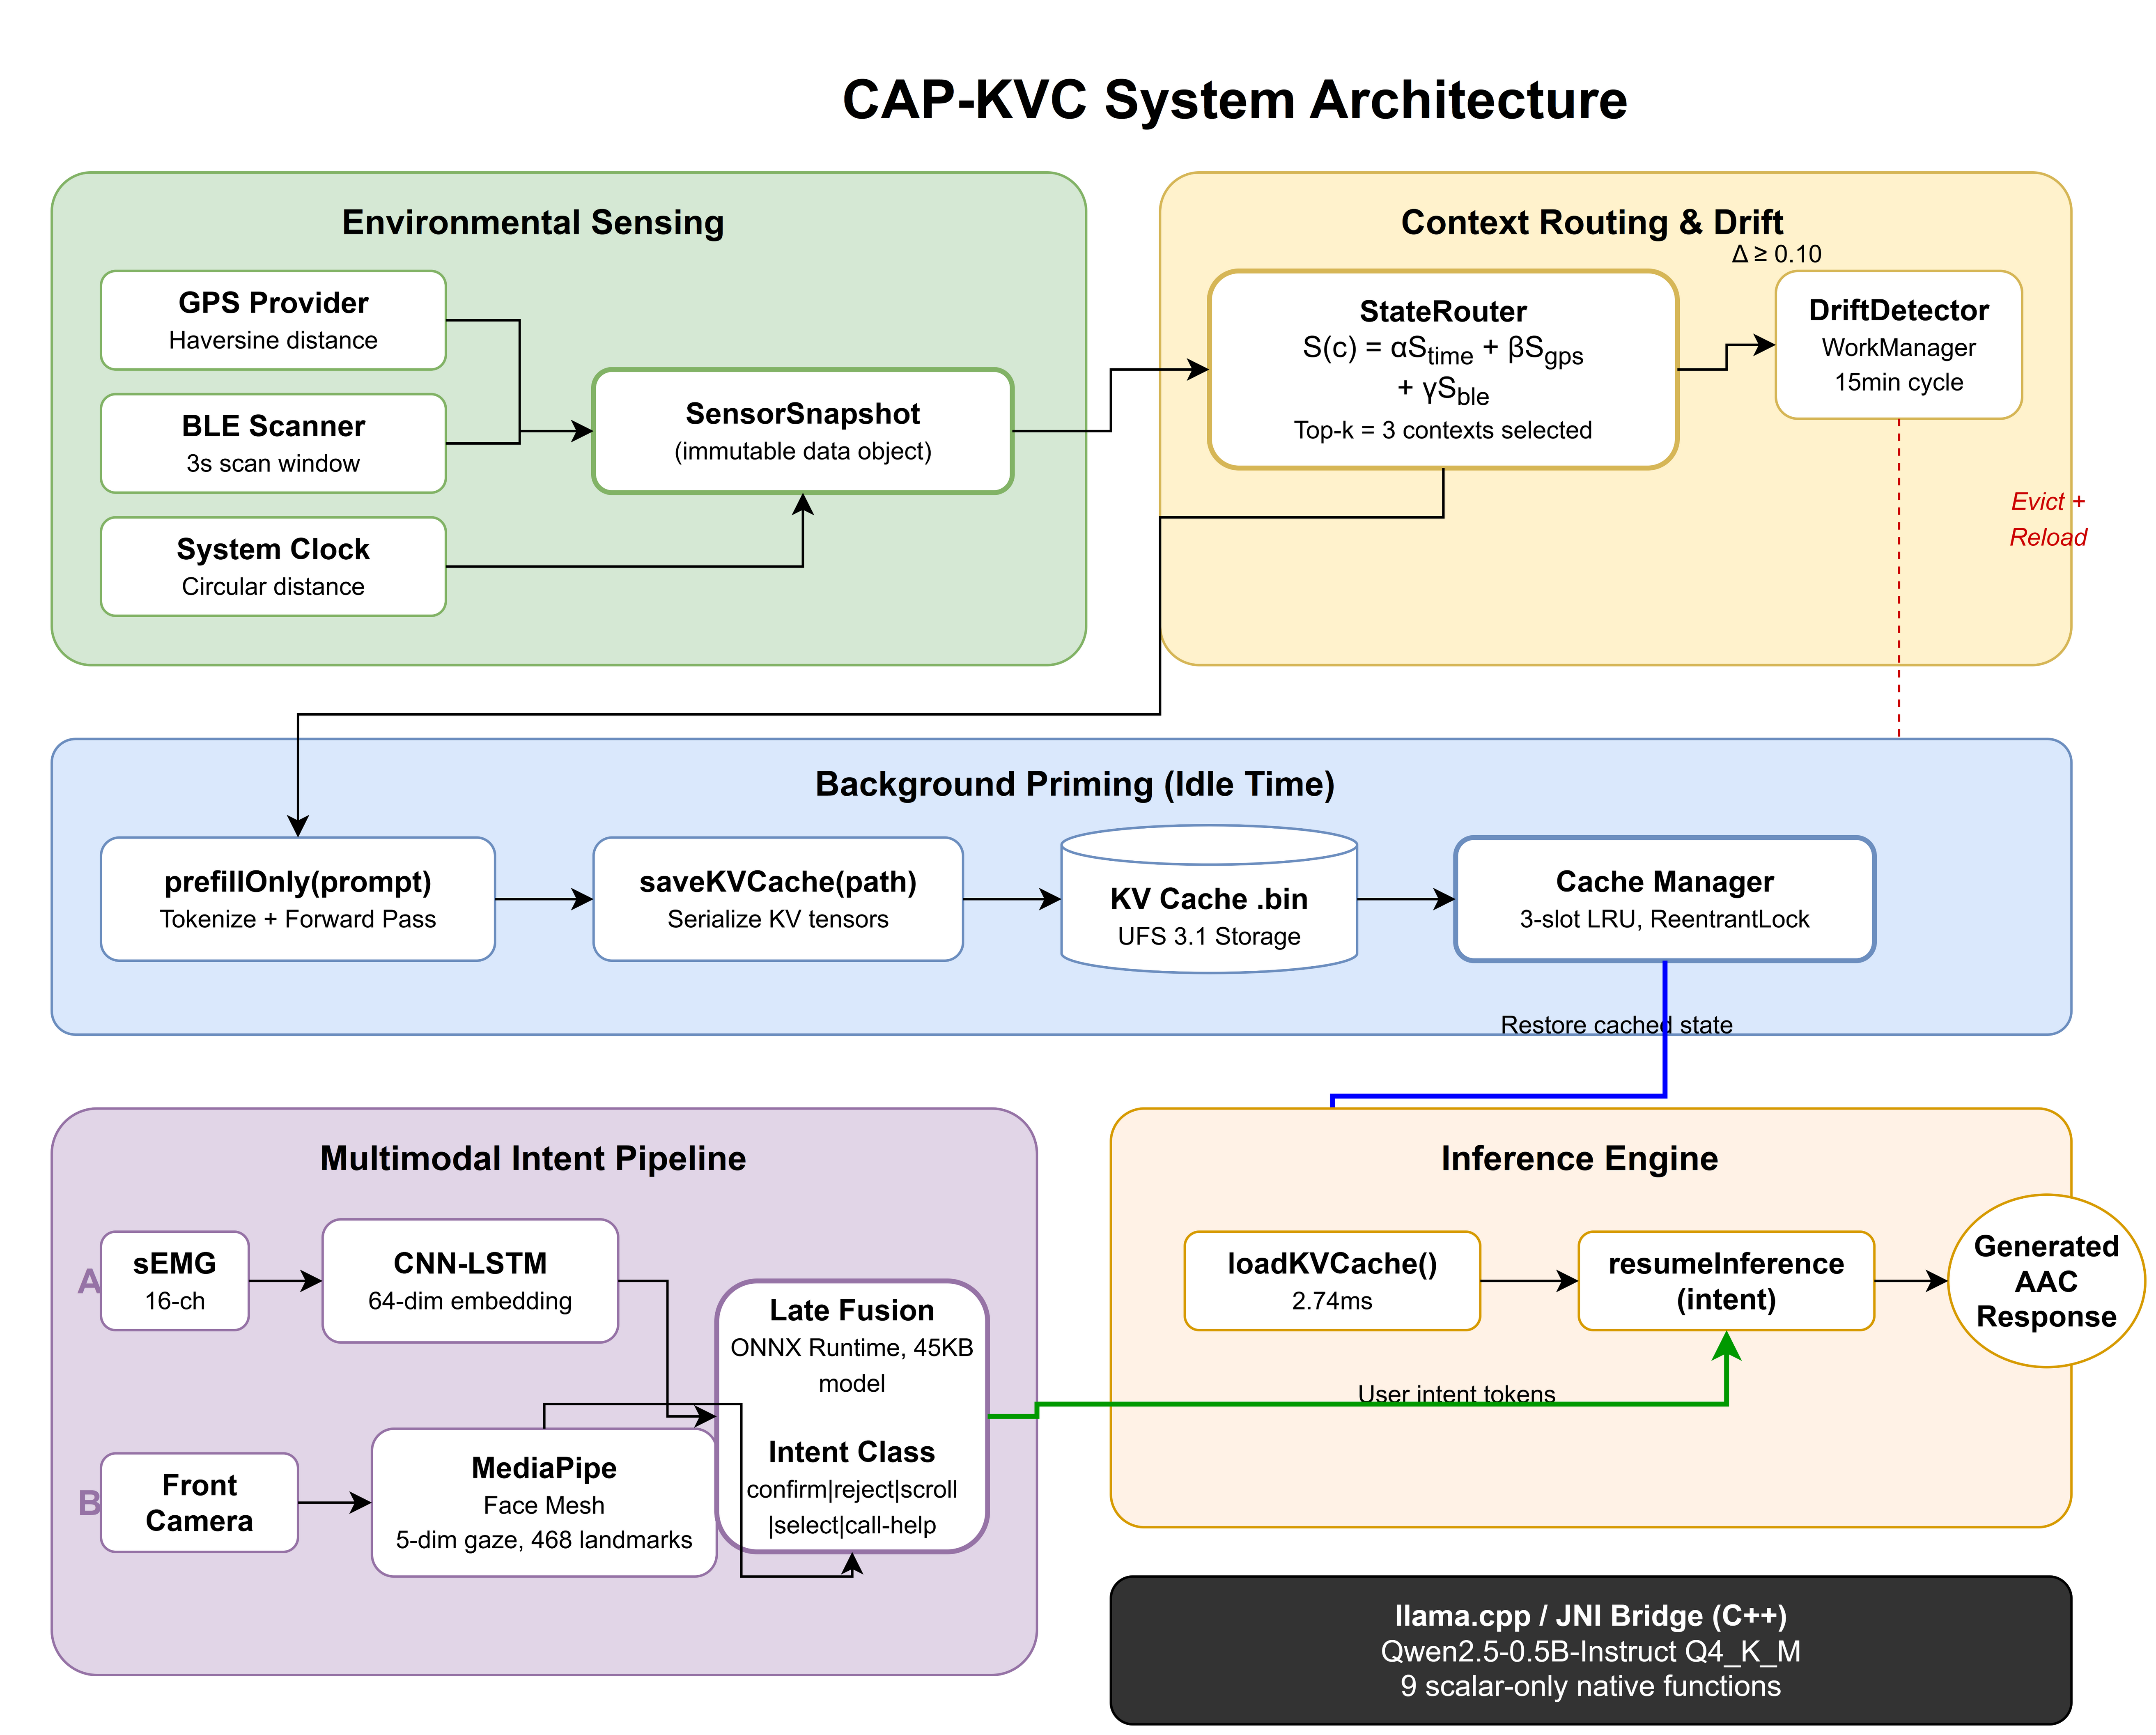
\includegraphics[width=\textwidth]{system_architecture_new.png}
\caption{CAP-KVC system architecture. Environmental sensors (blue) feed a scoring function selecting contexts for background priming (green). At inference time (orange), the pre-computed KV cache is restored and only intent tokens are processed by the llama.cpp/JNI backend. A drift detector re-evaluates context relevance with hysteresis gating ($\Delta \geq 0.10$).}
\label{fig:architecture}
\end{figure*}

\subsection{Problem Formulation}

Let $C = \{c_1, \ldots, c_M\}$ be a set of pre-configured semantic contexts, each associated with a system prompt $p_i$ of $N_i$ tokens. In standard retrieval-augmented generation, $p_i$ is concatenated with the user's intent tokens at inference time, incurring an $O(N_i)$ prefill cost. CAP-KVC reformulates this as a scheduling problem: predict the most likely context $\hat{c}$ from environmental signals, execute the prefill of $p_{\hat{c}}$ during idle periods, and persist the resulting KV cache tensors. At inference time, the system restores the pre-computed cache and appends only the user's intent tokens, reducing the inference-time cost from a prompt-length-dependent prefill to a cache restoration operation whose cost is independent of the original prompt length.

\subsection{Execution Pipeline}

The system operates in five stages. The first three run asynchronously during idle periods: (1)~\emph{sensor acquisition} polls GPS, BLE, and the system clock to construct an immutable \texttt{SensorSnapshot}; (2)~\emph{context routing} evaluates all registered contexts via a convex scoring function (Section~\ref{sec:scoring}) and selects the top-$k$ for cache residency; (3)~\emph{background priming} executes the prefill for each selected context, serializes the KV tensors, and registers the context as resident. At interaction time: (4)~\emph{resident inference} restores the pre-computed cache and appends only the intent tokens; (5)~\emph{drift correction} periodically re-evaluates scores and triggers cache replacement when a candidate exceeds the weakest resident state's score by at least $\Delta = 0.10$, preventing cache thrashing under noisy sensor conditions.

\subsection{Context Scoring}
\label{sec:scoring}

A context $c_i$ is scored as a convex combination of environmental similarity:
\begin{equation}
S(c_i) = \alpha \cdot S_{\text{time}} + \beta \cdot S_{\text{gps}} + \gamma \cdot S_{\text{ble}}
\label{eq:scoring}
\end{equation}
where $\alpha + \beta + \gamma = 1$. Temporal similarity applies a Gaussian kernel ($\sigma = 2.0$~h) over circular time distance:
\begin{equation}
S_{\text{time}} = \exp\!\left(-\frac{d_{\text{circ}}(t, t_i)^2}{2\sigma^2}\right)
\label{eq:time_score}
\end{equation}
Spatial similarity uses exponential decay over Haversine distance ($\lambda = 0.1$~km):
\begin{equation}
S_{\text{gps}} = \exp(-\lambda \cdot d_{\text{haversine}})
\label{eq:gps_score}
\end{equation}
BLE similarity evaluates device-topology overlap with sigmoid-mapped RSSI values. Weights are computed dynamically from sensor reliability: time maintains a fixed baseline $w_t = 0.4$, guaranteeing a positive normalization denominator even when both GPS and BLE are unavailable. GPS reliability decays exponentially with reported accuracy ($w_g = \exp(-a/50.0)$); BLE reliability derives from mean sigmoid-transformed RSSI centered at $-70$~dBm. Missing sensors receive zero weight and remaining weights are renormalized to preserve $\alpha + \beta + \gamma = 1$. Contexts scoring below 0.01 are excluded.

\subsection{KV Cache Residency}

The system maintains at most $k = 3$ KV cache states simultaneously resident in native memory, mapped to native sequence slots managed by the inference engine. When all slots are occupied, the LRU state is evicted. Eviction is protected by reference counting: a state under active inference holds a reference blocking eviction until inference completes. The eviction sequence marks the victim inactive, polls until its reference count drains to zero, and returns the native slot to the available pool.

% ===========================================================================
% IV. IMPLEMENTATION
% ===========================================================================
\section{Implementation}
\label{sec:implementation}

The system targets \texttt{arm64-v8a} devices running Android~12+, with \texttt{llama.cpp}~\cite{llamacpp} as the inference backend and Qwen2.5-0.5B-Instruct~\cite{qwen25} (Q4\_K\_M) as the evaluation model. Pre-compiled native libraries are bundled in the APK. All dependency injection is manual to minimize startup latency.

\textbf{JNI boundary.}
Nine native functions are exposed via JNI in a single C++ source file (801 lines), organized into three groups: lifecycle (\texttt{initializeBackend}, \texttt{initializeModel}, \texttt{release}), KV cache operations (\texttt{saveKVCache}, \texttt{loadKVCache}, \texttt{clearKVCache}), and inference (\texttt{runInference}, \texttt{prefillOnly}, \texttt{resumeInference}). A strict design constraint governs this boundary: \textbf{all arguments and return values are JNI scalar types} (\texttt{jstring}, \texttt{jint}, \texttt{jboolean})---no Java objects, arrays, or callbacks cross the boundary, eliminating GC root pinning. The critical distinction is between \texttt{runInference} (clears session, processes from position zero) and \texttt{resumeInference} (appends at position $n_{\text{past}}$), preventing position-ID collisions that would corrupt the attention computation.

\textbf{Concurrency.}
The C++ backend maintains shared global state (a \texttt{llama\_context} pointer and \texttt{session\_tokens} vector) accessed by the background priming coroutine, cache manager, and foreground inference path. A single \texttt{ReentrantLock} (the ``engine lock'') guards all JNI call sequences. The lock is held across both \texttt{loadKVCache} and \texttt{resumeInference} within a single acquisition, because releasing between calls would allow another thread to mutate \texttt{session\_tokens}. Per-state coroutine \texttt{Mutex} instances separately protect cache residency metadata without blocking unrelated cache operations.

\textbf{Cache priming lifecycle.}
Each state undergoes three phases: (1)~prefill via \texttt{prefillOnly} under the engine lock, which runs the forward pass without entering the generation loop; (2)~serialization via \texttt{saveKVCache} to a temporary file while still holding the lock (sequence slot~0 is mandatory since \texttt{prefillOnly} decodes into slot~0 via \texttt{llama\_batch\_get\_one}); (3)~atomic rename to the final path after lock release, exploiting ext4's atomic \texttt{rename()} to guarantee crash consistency. A model-readiness gate (\texttt{AtomicBoolean}) prevents priming before native context initialization.

\textbf{Sensor integration.}
Background sensing uses two cooperating components: an \emph{ActiveSweep} coroutine that concurrently acquires GPS coordinates (via cached \texttt{getLastKnownLocation}) and BLE topology (via a 3-second \texttt{BluetoothLeScanner} window), and a \emph{DriftDetector} \texttt{CoroutineWorker} registered with \texttt{WorkManager} for 15-minute periodic execution using a BLE-blind snapshot. A \texttt{BroadcastReceiver} for \texttt{BOOT\_COMPLETED} and \texttt{MY\_PACKAGE\_REPLACED} triggers cache population at boot via the \texttt{goAsync()} pattern.

\textbf{Inference fallback.}
If no cached context is available at interaction time (cold miss), a two-tier fallback fires: Tier~1 returns a generic pre-configured response immediately; Tier~2 initiates an asynchronous RAG prefill so subsequent intents can use contextual inference once the prefill completes.

% ===========================================================================
% V. EVALUATION
% ===========================================================================
\section{Evaluation}
\label{sec:experiments}

\subsection{Setup}

\textbf{Hardware.} OnePlus~11R (Snapdragon~8+~Gen~1, 8~GB LPDDR5X, UFS~3.1), Android~14, airplane mode, 50\% brightness, no other foreground applications.

\textbf{Model.} Qwen2.5-0.5B-Instruct Q4\_K\_M via \texttt{llama.cpp} GGUF (\texttt{n\_ctx}$=2048$, \texttt{n\_batch}$=512$, \texttt{n\_threads}$=4$, greedy decoding, max 64 output tokens).

\textbf{Conditions.} Three pipelines are compared: (1)~ZERO\_CONTEXT (intent tokens only, establishing the hardware latency floor); (2)~RAG\_INLINE (full context + intent via \texttt{runInference}, $N \in \{50, 100, 200, 500\}$); (3)~CAP\_KVC (restored cache via \texttt{loadKVCache} + intent via \texttt{resumeInference}). Each condition runs 32 sequential trials (2~warmup, 30~measured). The warmup phase absorbs Kotlin/ART JIT compilation and initial thermal settling.

\textbf{Important limitation.} CAP\_KVC caches were derived from $\sim$50-token prompts. Comparisons against longer RAG\_INLINE contexts characterize inference-time amortization behavior rather than response quality under equivalent context richness.

\subsection{Measurement Methodology}
\label{sec:measurement}

End-to-end wall-clock latency is captured via \texttt{System.nanoTime()} at the Kotlin layer. To decompose latency into constituent phases, \texttt{std::chrono::high\_resolution\_clock} timestamps are inserted immediately before and after each \texttt{llama\_decode()} call within both \texttt{runInference} and \texttt{resumeInference}. This isolates the prefill phase---the single \texttt{llama\_decode()} call that processes all prompt tokens---from the autoregressive generation loop. On the Android NDK runtime, \texttt{high\_resolution\_clock} maps to the monotonic \texttt{CLOCK\_MONOTONIC} source (vDSO-accelerated, $\approx$10--50~ns overhead), preventing corruption from NTP synchronization. JNI boundaries and log serialization occur strictly outside the timed regions.

For the CAP\_KVC condition, three sub-components are instrumented separately: \texttt{cache\_load\_ms} (Kotlin layer), \texttt{prefill\_ms} (native layer, intent-only \texttt{llama\_decode}), and \texttt{gen\_ms} (native layer, generation loop). Both layers are captured under the same engine lock acquisition.

Results are emitted as structured CSV via \texttt{adb logcat}. The extraction script matches JNI timing entries to Kotlin bench entries by strict proximity and asserts alignment of trial indices and token counts; any mismatch aborts the parser. All 180 trials reported here were fully verified.

% ===========================================================================
% VI. RESULTS
% ===========================================================================
\section{Results}
\label{sec:results}

\subsection{Inference Latency}
\label{sec:results_latency}

Table~\ref{tab:latency} reports latency with native-side prefill decomposition ($n = 30$ per condition, 180 total).

\begin{table}[htbp]
\centering
\caption{Latency decomposition (ms). Prefill isolates the \texttt{llama\_decode()} forward pass; generation covers autoregressive sampling. Both measured via native \texttt{std::chrono}. OnePlus~11R, Qwen2.5-0.5B-Instruct Q4\_K\_M, greedy sampling, max 64~output tokens, $n = 30$.}
\label{tab:latency}
\resizebox{\columnwidth}{!}{%
\begin{tabular}{lrrrrr}
\hline
\textbf{Condition} & \textbf{E2E (ms)} & \textbf{Prefill (ms)} & \textbf{Gen (ms)} & \textbf{E2E $\sigma$} & \textbf{Tokens} \\
\hline
ZERO\_CONTEXT       & 3823.78 & 274.79  & 3544.58  & 569.76  & 9  \\
RAG ($N\!\approx\!50$)  & 6547.13 & 2021.46 & 4508.53  & 8392.58 & 52 \\
RAG ($N\!\approx\!100$) & 7900.92 & 3015.09 & 4877.95  & 3857.18 & 89 \\
RAG ($N\!\approx\!200$) & 12122.30 & 6673.53 & 5439.96 & 2740.12 & 206 \\
RAG ($N\!\approx\!500$) & 19408.89 & 14001.46 & 5390.76 & 2113.04 & 439 \\
\hline
CAP\_KVC (cache load)       & 2.74  & ---  & ---  & 1.35 & --- \\
CAP\_KVC (inference)        & 4571.97 & 343.35 & 4226.74  & 373.65 & 9  \\
CAP\_KVC (total)            & 4574.70 & ---    & ---      & 373.49 & ---  \\
\hline
\end{tabular}%
}
\end{table}

\begin{figure}[htbp]
\centering
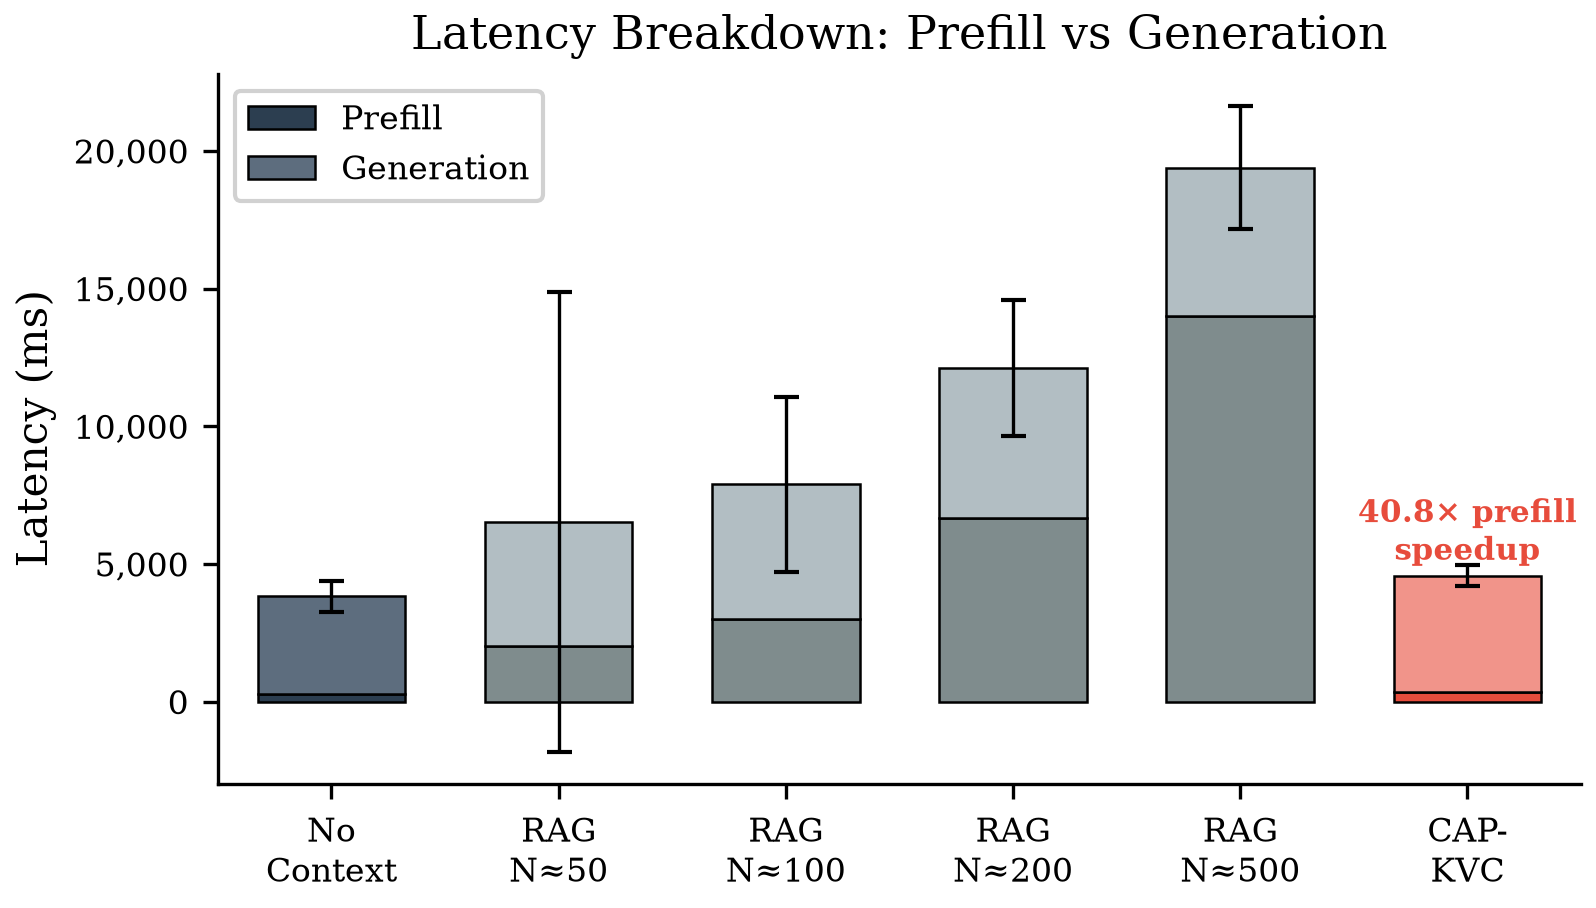
\includegraphics[width=\columnwidth]{latency_breakdown_new.png}
\caption{Latency decomposition across conditions. RAG\_INLINE prefill scales linearly (274~ms at $N\!=\!9$ to 14001~ms at $N\!=\!439$ tokens); CAP\_KVC prefill is 343~ms regardless of cached context size, yielding a 40.78$\times$ prefill speedup. Error bars: $\pm 1\sigma$, $n = 30$.}
\label{fig:latency_breakdown}
\end{figure}

\textbf{Cache restoration is negligible.} The mean cache load time is 2.74~ms ($\sigma = 1.35$~ms), representing less than 0.1\% of total CAP\_KVC latency. This measures the complete Kotlin-side \texttt{loadKVCache()} round trip including JNI marshalling, native file I/O, and KV tensor deserialization.

\textbf{Prefill amortization.} RAG\_INLINE prefill scales linearly from 2021~ms ($N \approx 52$) to 14001~ms ($N \approx 439$), a 6.93$\times$ increase. CAP\_KVC prefill is 343.35~ms ($\sigma = 45.00$~ms) for 9 intent tokens regardless of cached context size, yielding a \textbf{40.78$\times$ prefill speedup} at $N \approx 500$. End-to-end, CAP\_KVC achieves 4574.70~ms versus 19408.89~ms, a \textbf{4.24$\times$ speedup}. The generation phase ($\sim$3500--5400~ms) masks the prefill improvement in the end-to-end ratio.

\textbf{Statistical significance.} Welch's two-sample $t$-tests ($\alpha = 0.05$, two-tailed) on prefill-only latency confirm significance: CAP\_KVC vs.\ RAG@500 ($t(29.0) = -40.42$, $p < 10^{-26}$, Cohen's $d = 10.44$); CAP\_KVC vs.\ RAG@50 ($p = 0.011$, $d = 0.70$, medium-to-large effect). The end-to-end comparison at $N \approx 500$ is also significant ($t(30.8) = -37.86$, $p < 10^{-26}$, $d = 9.78$); at $N \approx 50$ it is not ($p = 0.209$) due to high generation-phase variance. Although Welch's $t$-test is robust to unequal variances, the extreme skewness of RAG latency distributions violates normality assumptions; the reported statistics should be interpreted as general trends.

\textbf{Generation-phase variance.} Generation time varies across conditions (ZERO\_CONTEXT 3544~ms, RAG@500 5390~ms, CAP\_KVC 4226~ms), consistent with differing per-token attention cost when the KV cache contains different numbers of entries and with uncharacterized system-level effects over the 29-minute benchmark session. Because prefill and generation are decomposed independently, these differences do not confound the prefill speedup.

\textbf{Outliers.} Five trials were flagged by Tukey's criterion ($Q_3 + 3 \times \text{IQR}$). No thermal telemetry or CPU frequency logs were captured, so the specific mechanisms cannot be attributed. All outliers were retained in reported statistics to preserve operational realism.

\subsection{Memory Budget}
\label{sec:results_memory}

\begin{table}[htbp]
\centering
\caption{Native heap memory (KB) via \texttt{dumpsys meminfo}. Delta represents the marginal cost of loading three KV cache states.}
\label{tab:memory}
\begin{tabular}{lrr}
\hline
\textbf{State} & \textbf{Native Heap (KB)} & \textbf{Total PSS (KB)} \\
\hline
Idle (0 states)     & 18,856  & 623,488 \\
Loaded (3 states)   & 140,420 & 612,940 \\
\hline
\textbf{Delta}      & +121,564 ($\approx$118.7~MB) & --- \\
\hline
\end{tabular}
\end{table}

Three-state residency adds approximately 118.7~MB of native heap ($\sim$40~MB per state for a 0.5B Q4\_K\_M model), a feasible budget on 8~GB devices. The slight PSS decrease between states reflects measurement variability in shared memory attribution.

\subsection{Multimodal Fusion (Proof-of-Concept)}
\label{sec:results_fusion}

As a motivating application interface, a late fusion model combining CNN-LSTM sEMG embeddings ($\mathbb{R}^{64}$) with MediaPipe gaze features ($\mathbb{R}^{5}$) was evaluated on a synthetic dataset (2000 paired samples, 60/20/20 split). The pre-specified decision criterion required the cross-attention model to exceed late fusion F1 by more than 3~percentage points (absolute). Late fusion achieves macro F1 = 0.9963 versus cross-attention F1 = 0.9437 (5.26~pp difference, reversed direction), so the simpler architecture was selected. The standalone CNN-LSTM EMG classifier achieves 42.4\% accuracy under cross-subject LOSO evaluation (NinaPro~DB5~\cite{ninapro}), with 0\% recall on the \emph{reject} class---expected given inter-subject EMG variability. These numbers characterize model capacity on synthetic/controlled data and do not predict clinical accuracy; no gaze-only baseline was evaluated.

\subsection{Drift Detection}
\label{sec:results_drift}

An offline Sentence-BERT k-ablation on DailyDialog~\cite{dailydialog} yields maximum F1 = 0.367 at $k = 1$, degrading monotonically with window size. The deployed system uses $k = 3$ as a sensor-score smoothing heuristic---chosen for stability against transient sensor fluctuations rather than from the DailyDialog results, which are methodologically distinct (Sentence-BERT centroid distances vs.\ deployed sensor-score hysteresis).

% ===========================================================================
% VII. CONCLUSION AND LIMITATIONS
% ===========================================================================
\section{Conclusion}
\label{sec:conclusion}

CAP-KVC demonstrates that sensor-driven predictive caching eliminates prompt-length-dependent prefill latency on mobile hardware. Native-side instrumentation confirms a 40.78$\times$ prefill speedup (343~ms vs.\ 14001~ms at $N \approx 500$) and 4.24$\times$ end-to-end reduction (4574~ms vs.\ 19408~ms), with 2.74~ms cache restoration. The Android implementation operates within 118.7~MB native heap for three simultaneous cache states. The approach generalizes beyond the AAC motivating scenario: any mobile application processing recurring environmental contexts can exploit idle-time cache priming.

\textbf{Limitations.}
All benchmarks use a single device (OnePlus~11R, Snapdragon~8+~Gen~1) and a single model (Qwen2.5-0.5B Q4\_K\_M) with $n = 30$ trials; results may differ on other SoCs or model families. The fusion evaluation uses synthetic data and lacks clinical validation or a gaze-only baseline. Prefill timing measures the single \texttt{llama\_decode()} call; tokenization overhead ($< 1$~ms) is excluded. No thermal telemetry, CPU frequency logs, power measurements, or non-predictive cache baseline were captured. The evaluation uses five static context configurations rather than learned profiles. Serialized KV cache files are unencrypted, relying on Android's application sandbox. Battery impact of the \texttt{ContextDaemon} (60-second sweep) and \texttt{DriftDetector} (15-minute poll via WorkManager) has not been characterized.

% ===========================================================================
% REFERENCES
% ===========================================================================
\begin{thebibliography}{20}

\bibitem{beukelman2020}
D.~R. Beukelman and J.~C. Light,
``Augmentative and alternative communication,''
\emph{Paul H. Brookes Publishing}, 5th ed., 2020.

\bibitem{llamacpp}
G.~Gerganov,
``llama.cpp: LLM inference in {C/C++},''
2023. [Online]. Available: \url{https://github.com/ggerganov/llama.cpp}

\bibitem{qwen25}
A.~Yang \emph{et al.},
``{Qwen2.5 Technical Report},''
\emph{arXiv:2412.15115}, 2024.

\bibitem{dettmers2022}
T.~Dettmers, M.~Lewis, Y.~Belkada, and L.~Zettlemoyer,
``{LLM.int8()},''
in \emph{Proc. NeurIPS}, 2022.

\bibitem{frantar2022}
E.~Frantar, S.~Ashkboos, T.~Hoefler, and D.~Alistarh,
``{GPTQ},''
in \emph{Proc. ICLR}, 2023.

\bibitem{scissorhands}
Z.~Liu \emph{et al.},
``Scissorhands,''
in \emph{Proc. NeurIPS}, 2023.

\bibitem{h2o}
Z.~Zhang \emph{et al.},
``{H$_2$O},''
in \emph{Proc. NeurIPS}, 2023.

\bibitem{streamingllm}
G.~Xiao, Y.~Tian, B.~Chen, S.~Han, and M.~Lewis,
``{Efficient streaming language models with attention sinks},''
\emph{arXiv:2309.17453}, 2023.

\bibitem{sglang}
L.~Zheng \emph{et al.},
``{SGLang},''
in \emph{Proc. NeurIPS}, 2024.

\bibitem{vllm}
W.~Kwon \emph{et al.},
``{PagedAttention},''
in \emph{Proc. 29th SOSP}, 2023.

\bibitem{infinigen}
W.~Lee, J.~Lee, J.~Seo, and J.~Sim,
``{InfiniGen},''
in \emph{Proc. 18th USENIX OSDI}, 2024.

\bibitem{cachegen}
Y.~Liu \emph{et al.},
``{CacheGen},''
in \emph{Proc. ACM SIGCOMM}, 2024.

\bibitem{ninapro}
M.~Atzori \emph{et al.},
``{NinaPro},''
\emph{Scientific Data}, vol.~1, p.~140053, 2014.

\bibitem{snapkv}
Y.~Li \emph{et al.},
``{SnapKV},''
\emph{arXiv:2404.14469}, 2024.

\bibitem{promptcache}
I.~Gim \emph{et al.},
``{Prompt Cache},''
in \emph{Proc. MLSys}, 2024.

\bibitem{cacheblend}
J.~Yao \emph{et al.},
``{CacheBlend},''
\emph{arXiv:2405.16444}, 2024.

\bibitem{powerinfer2}
Z.~Xue \emph{et al.},
``{PowerInfer-2},''
\emph{arXiv:2406.06282}, 2024.

\bibitem{kvquant}
C.~Hooper \emph{et al.},
``{KVQuant},''
in \emph{Proc. NeurIPS}, 2024.

\bibitem{mobilellm}
Z.~Liu \emph{et al.},
``{MobileLLM},''
in \emph{Proc. ICML}, 2024.

\bibitem{mlcllm}
MLC Team,
``{MLC LLM},''
2023. [Online]. Available: \url{https://github.com/mlc-ai/mlc-llm}

\bibitem{llminaflash}
K.~Alizadeh \emph{et al.},
``{LLM in a Flash},''
\emph{arXiv:2312.11514}, 2023.

\bibitem{vaswani2017}
A.~Vaswani \emph{et al.},
``{Attention is all you need},''
in \emph{Proc. NeurIPS}, 2017.

\bibitem{dailydialog}
Y.~Li \emph{et al.},
``{DailyDialog},''
\emph{arXiv:1710.03957}, 2017.

\end{thebibliography}

\end{document}
